% 1986 年上海卷文史类第 7 题：抛物线与圆的交点及弦中点
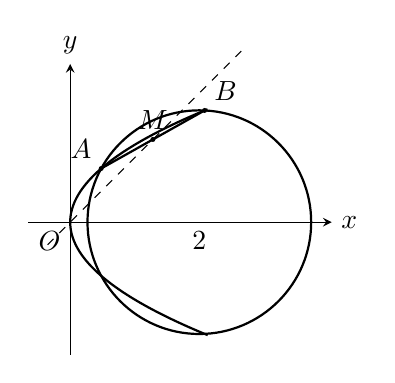
\begin{tikzpicture}[scale=0.82,>=stealth]
  \draw[->] (-0.65,0)--(4.05,0) node[right] {$x$};
  \draw[->] (0,-2.05)--(0,2.45) node[above] {$y$};
  \draw[thick] (2,0) circle (1.732);
  \draw[thick,domain=-1.75:1.75,samples=100]
    plot ({\x*\x/1.438},{\x});
  \draw[dashed] (-0.35,-0.35)--(2.65,2.65);
  \draw[thick] (0.480,0.831)--(2.081,1.730);
  \fill (0.480,0.831) circle (1.1pt) node[above left] {$A$};
  \fill (2.081,1.730) circle (1.1pt) node[above right] {$B$};
  \fill (1.281,1.281) circle (1.1pt) node[above] {$M$};
  \node[below left] at (0,0) {$O$};
  \node[below] at (2,0) {$2$};
\end{tikzpicture}
